% --- KHAI BÁO CÁC ĐỊNH NGHĨA DÙNG CHUNG (Đặt ở đây để Section nào cũng dùng được) ---

% --- ĐỊNH NGHĨA MÀU ---
\definecolor{customBlueTitle}{HTML}{6FA8DC}
\definecolor{customBlueBody}{HTML}{CFE2F3}
\definecolor{customGreenTitle}{HTML}{70AD47}
\definecolor{customGreenBody}{HTML}{B6D7A8}
\definecolor{customGreenCardBG}{HTML}{D9EAD3}
\definecolor{headerBlue}{HTML}{6FA8DC} % Màu cho bảng so sánh



% --- ĐƯỜNG DẪN ẢNH (Lưu ý đường dẫn tuyệt đối của bạn) ---
\newcommand{\pathIcons}{images/TongQuan/icons/}
\newcommand{\pathImages}{images/TongQuan/}

% --- MACRO VẼ THẺ TIKZ ---
\newcommand{\drawCustomCard}[2]{%
    \begin{tikzpicture}
        \def\cardW{3.45cm}%
        \def\totalH{2.15cm}%
        \def\splitY{1.2cm}%
        \def\rad{0.2cm}%
        \def\imgH{0.95cm}%
        % --- PHẦN 1: ẢNH ---
        \begin{scope}
            \clip [rounded corners=\rad] (0,\splitY) -- (\cardW,\splitY) -- (\cardW,\totalH) -- (0,\totalH) -- cycle;
            \node[anchor=south west, inner sep=0] at (0,\splitY) {
                \includegraphics[width=\cardW, height=\imgH, keepaspectratio=false]{#1}
            };
        \end{scope}
        % --- PHẦN 2: TEXT ---
        \begin{scope}
            \path[fill=customGreenCardBG, rounded corners=\rad] (0,0) -- (\cardW,0) -- (\cardW,\splitY) -- (0,\splitY) -- cycle;
            \node[anchor=center] at (\cardW/2, \splitY/2) {
                \begin{minipage}{3.25cm}
                    \centering
                    \fontsize{5}{6}\selectfont 
                    \color{black} 
                    #2
                \end{minipage}
            };
        \end{scope}
    \end{tikzpicture}%
}



%------------------------------------------------
\section{Cơ sở lý thuyết \& tổng quan}
\SectionIntro{Phần 2: Cơ sở lý thuyết \& tổng quan}{Các khái niệm cơ bản và bài toán phát hiện lỗi.}

%------------------------------------------------
% \begin{frame}
% \label{Maths}
% 	\frametitle{TỔNG QUAN TẤM PIN NĂNG LƯỢNG MẶT TRỜI}
% 	\begin{center}
% 		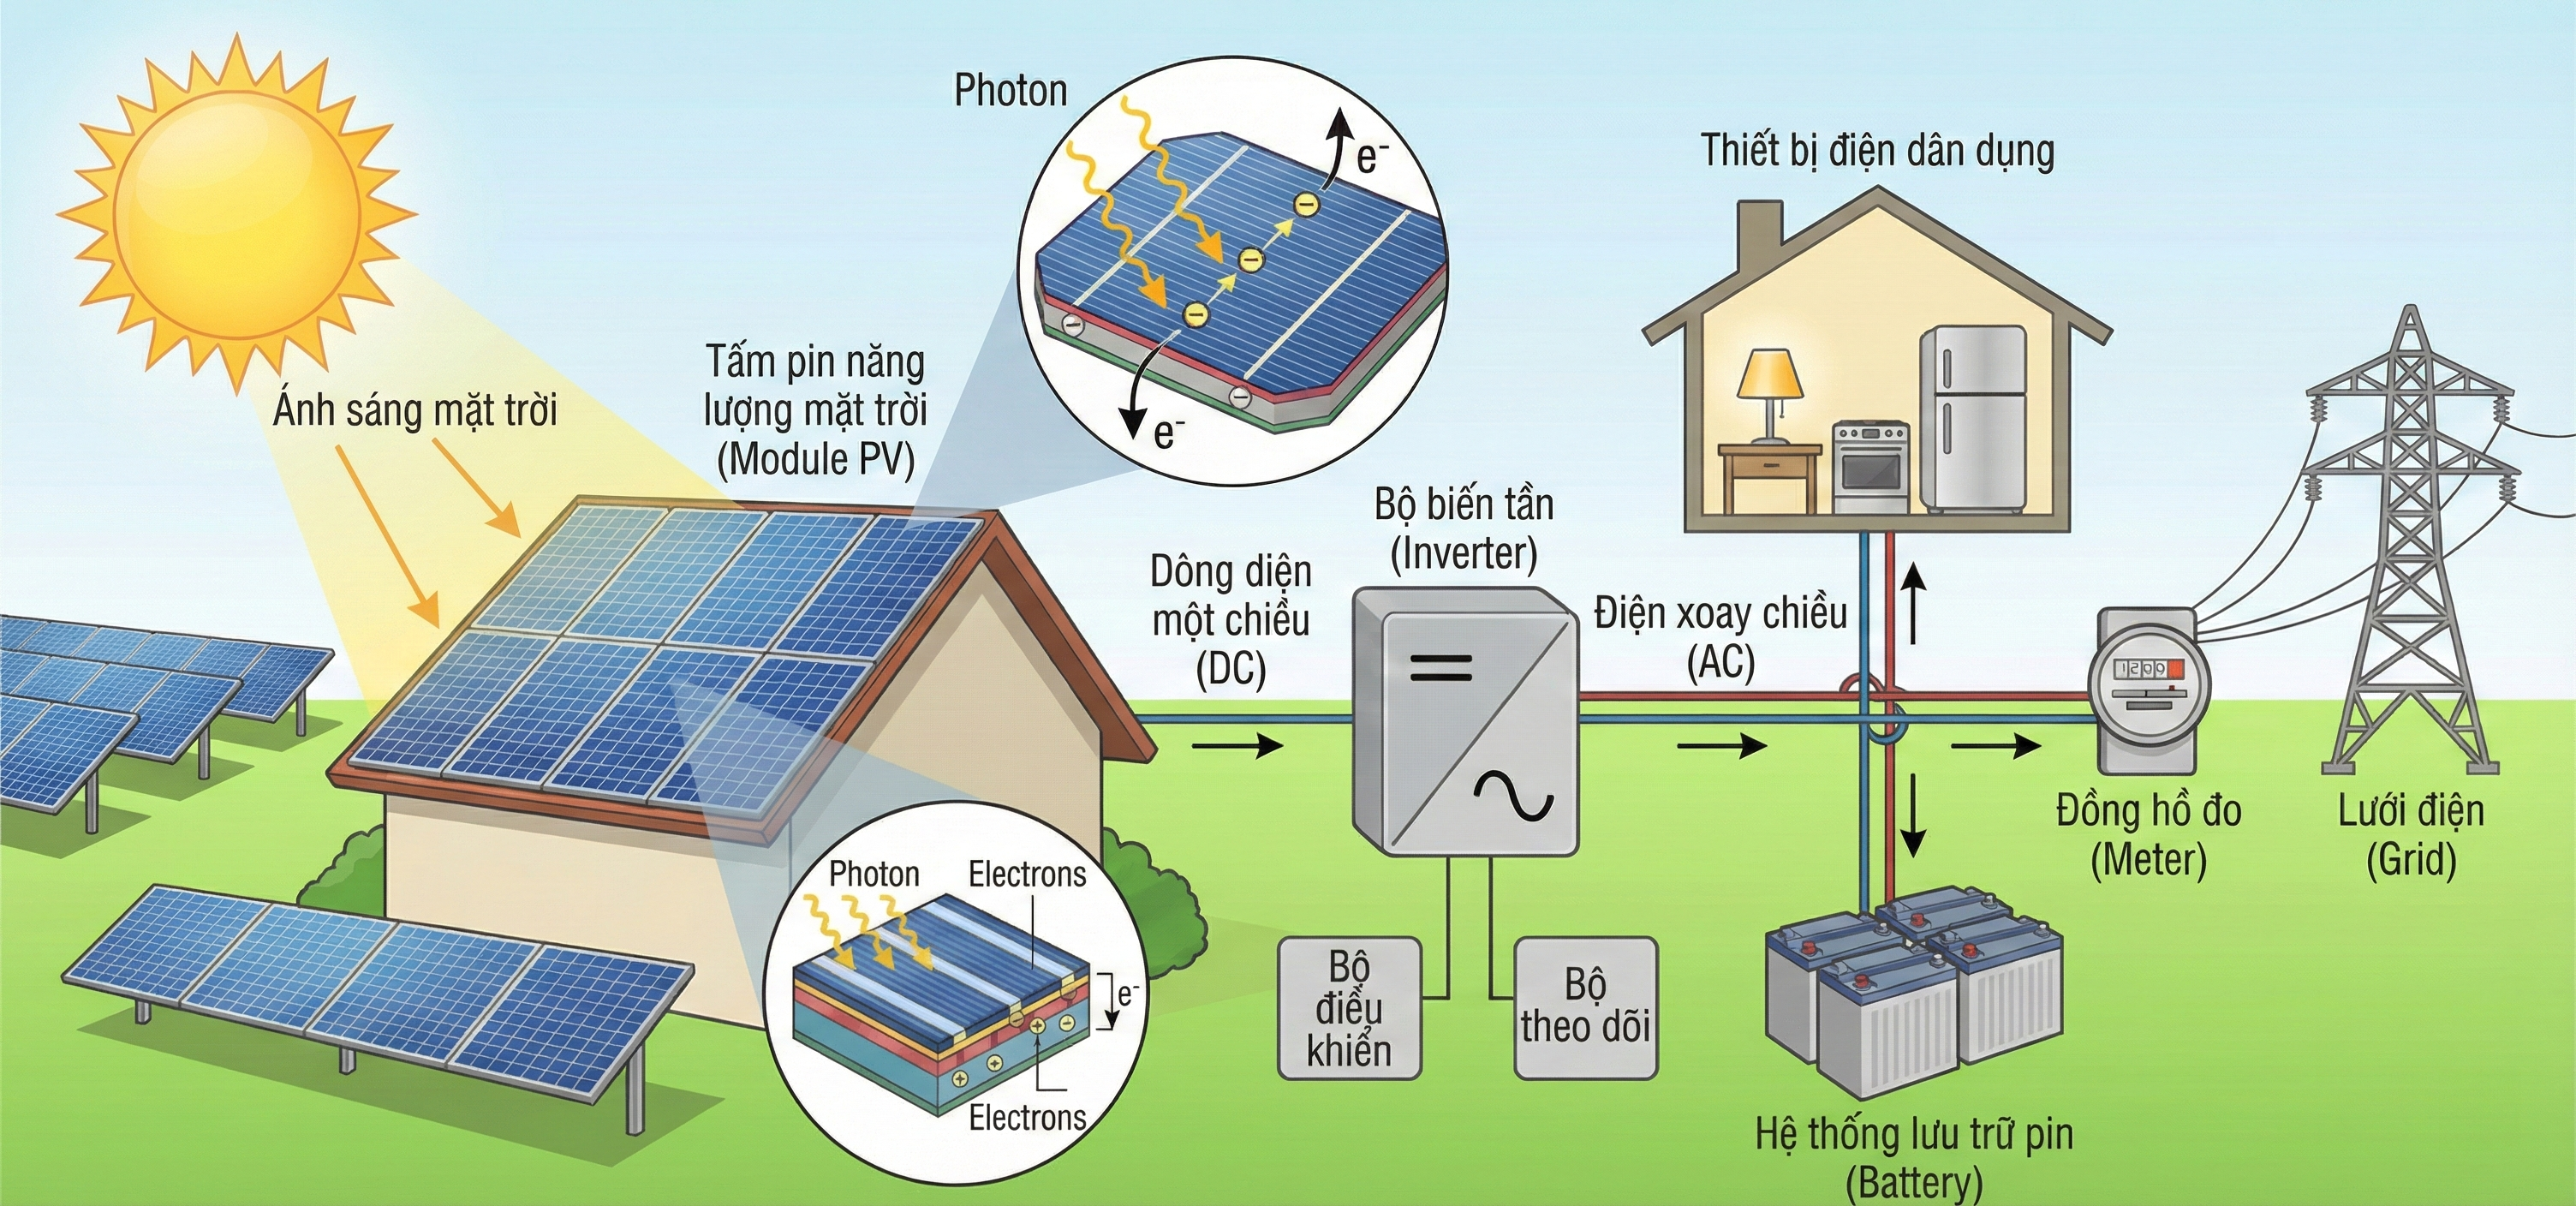
\includegraphics[width=0.8\textwidth]{images/TongQuan/pinmattroi.png}
% 	\end{center}
% \end{frame}

%------------------------------------------------
% SLIDE 10: ẨN - Tổng quan tiềm năng (đã gộp vào slide 11)
% \begin{frame}
% 	\frametitle{TÌNH HÌNH HỆ THỐNG PIN MẶT TRỜI TRÊN THẾ GIỚI}
% 	
% 	\vspace{0.3cm}
% 	
% 	\begin{columns}[t]
% 		% Cột 1: BÙNG NỔ
% 		\begin{column}{0.3\textwidth}
% 			\centering
% 			\includegraphics[width=0.5\textwidth]{images/TongQuan/icons/bungno.png}
% 			
% 			\vspace{0.3cm}
% 			
% 			{\Large\textbf{BÙNG NỔ}}
% 			
% 			\vspace{0.4cm}
% 			
% 			\small
% 			Diện mặt trời chiếm \\
% 			\textcolor{orange}{\textbf{73\%}} tổng công suất \\
% 			năng lượng tái tạo \\
% 			tăng thêm toàn cầu \\
% 			năm 2023.
% 		\end{column}
% 
% 		\vrule width 1pt
% 		
% 		% Cột 2: CHI PHÍ
% 		\begin{column}{0.3\textwidth}
% 			\centering
% 			\includegraphics[width=0.5\textwidth]{images/TongQuan/icons/chiphi.png}
% 			
% 			\vspace{0.3cm}
% 			
% 			{\Large\textbf{CHI PHÍ}}
% 			
% 			\vspace{0.4cm}
% 			
% 			\small
% 			Chi phí lắp đặt đã giảm sâu \\
% 			\textcolor{orange}{\textbf{85\%}} sau một thập kỷ, trở \\
% 			thành nguồn năng lượng \\
% 			dễ tiếp cận nhất.
% 		\end{column}
% 
% 		\vrule width 1pt
% 		
% 		% Cột 3: TIỀM NĂNG
% 		\begin{column}{0.3\textwidth}
% 			\centering
% 			\includegraphics[width=0.5\textwidth]{images/TongQuan/icons/tiemnang.png}
% 			
% 			\vspace{0.3cm}
% 			
% 			{\Large\textbf{TIỀM NĂNG}}
% 			
% 			\vspace{0.4cm}
% 			
% 			\small
% 			Việt Nam nằm trong \\
% 			``vùng đỏ'' bức xạ nhiệt, \\
% 			mang hữu tiềm năng tự \\
% 			nhiên lý tưởng để phát \\
% 			triển điện mặt trời.
% 		\end{column}
% 	\end{columns}
% 	
% \end{frame}

% SLIDE 11: GIỮ LẠI - Biểu đồ tăng trưởng (ấn tượng nhất)


% SLIDE 12: ẨN - Biểu đồ chi phí
% \begin{frame}
% \label{Chiphi}
% 	\frametitle{TÌNH HÌNH HỆ THỐNG PIN MẶT TRỜI TRÊN THẾ GIỚI}
% 	\begin{center}
% 		\includegraphics[width=0.6\textwidth]{images/TongQuan/bieudochiphi.png}
% 	\end{center}
% \end{frame}

% SLIDE 13: ẨN - Bản đồ bức xạ thế giới
% \begin{frame}
% \label{Nhiet}
% 	\frametitle{TÌNH HÌNH HỆ THỐNG PIN MẶT TRỜI TRÊN THẾ GIỚI}
% 	\begin{center}
% 		\includegraphics[width=0.8\textwidth]{images/TongQuan/bieudonhiet.png}
% 	\end{center}
% \end{frame}



% Định nghĩa màu nền xanh
\definecolor{CardBlue}{HTML}{B1CDFC}

% \begin{frame}
%     \frametitle{TÌNH HÌNH HỆ THỐNG PIN MẶT TRỜI TẠI VIỆT NAM}
%     \vspace{-0.85cm}
    
%     \begin{columns}[t, onlytextwidth]
%         \tcbset{
%             mycardstyle/.style={
%                 colback=white,
%                 colframe=gray!50,
%                 arc=6pt,
%                 boxrule=1pt,
%                 left=2pt, right=2pt, top=1pt, bottom=1pt,
%                 equal height group=A,
%                 fontupper=\scriptsize,
%                 halign=center,
%                 valign=top
%             }
%         }

%         % --- Card 1 ---
%         \begin{column}{0.31\textwidth}
%             \begin{tcolorbox}[mycardstyle]
%                 \begin{minipage}[t][2.95cm][t]{\linewidth}
%                     \raggedright
%                     % Tiêu đề
%                     \centering
%                     {\bfseries\small ĐIỆN MẶT TRỜI\\QUY MÔ LỚN}
                    
%                     \vspace{0.15cm}
%                     \raggedright
%                     \textbullet\ Nguồn cung cấp sản lượng điện lớn đóng góp vào lưới điện quốc gia.\\[0.05cm]
%                     \textbullet\ Các dự án kỷ lục: nhà máy Dầu Tiếng, tổ hợp Trung Nam.
%                 \end{minipage}
                
%                 % Yêu cầu 2: Ảnh bo góc bằng TikZ Clip
%                 \begin{tikzpicture}
%                     \clip [rounded corners=6pt] (0,0) rectangle (\linewidth, 2.2cm); 
%                     \node[anchor=south west, inner sep=0] at (0,0) {\includegraphics[width=\linewidth, height=2.2cm]{images/TongQuan/trungnam.jpg}};
%                 \end{tikzpicture}
%             \end{tcolorbox}
%         \end{column}\hfill

%         % --- Card 2 ---
%         \begin{column}{0.31\textwidth}
%             \begin{tcolorbox}[mycardstyle]
%                 \begin{minipage}[t][2.95cm][t]{\linewidth}
%                     \raggedright
%                     \centering
%                     {\bfseries\small ĐIỆN MẶT TRỜI\\ÁP MÁI}
                    
%                     \vspace{0.15cm}
%                     \raggedright
%                     \textbullet\ Tận dụng mái nhà xưởng và hộ gia đình.\\[0.05cm]
%                     \textbullet\ Ưu tiên hàng đầu: không tốn đất, giảm tải tại chỗ cho lưới điện.
%                 \end{minipage}
                
%                 \begin{tikzpicture}
%                     \clip [rounded corners=6pt] (0,0) rectangle (\linewidth, 2.2cm);
%                     \node[anchor=south west, inner sep=0] at (0,0) {\includegraphics[width=\linewidth, height=2.2cm]{images/TongQuan/apmai.png}};
%                 \end{tikzpicture}
%             \end{tcolorbox}
%         \end{column}\hfill

%         % --- Card 3 ---
%         \begin{column}{0.31\textwidth}
%             \begin{tcolorbox}[mycardstyle]
%                 \begin{minipage}[t][2.95cm][t]{\linewidth}
%                     \raggedright
%                     \centering
%                     {\bfseries\small ĐIỆN MẶT TRỜI\\ĐỘC LẬP}
                    
%                     \vspace{0.15cm}
%                     \raggedright
%                     \textbullet\ Khu vực chưa có điện lưới hoặc công trình độc lập.\\[0.05cm]
%                     \textbullet\ Cần tính toán kỹ pin lưu trữ để đảm bảo ổn định.
%                 \end{minipage}
                
%                 \begin{tikzpicture}
%                     \clip [rounded corners=6pt] (0,0) rectangle (\linewidth, 2.2cm);
%                     \node[anchor=south west, inner sep=0] at (0,0) {\includegraphics[width=\linewidth, height=2.2cm]{images/TongQuan/doclap.png}};
%                 \end{tikzpicture}
%             \end{tcolorbox}
%         \end{column}\hfill
        
%     \end{columns}

% \end{frame}

% Định nghĩa màu sắc giống trong ảnh
\definecolor{mypaleblue}{RGB}{189, 215, 238} % Màu xanh nhạt cho đường kẻ
\definecolor{myorange}{RGB}{197, 90, 17}    % Màu cam đậm cho tiêu đề (nếu cần)
\definecolor{myblueicon}{RGB}{0, 112, 192}  % Màu xanh cho icon

% --- KHAI BÁO LỆNH BO GÓC BẰNG TIKZ (ĐẶT NGOÀI FRAME) ---
% Nguyên lý: Vẽ 1 ảnh tàng hình để lấy kích thước -> Tạo khung cắt bo tròn -> Vẽ ảnh thật đè lên
\newcommand{\roundimg}[2]{ % Tham số: #1 = chiều cao, #2 = đường dẫn ảnh
    \begin{tikzpicture}[baseline=(img.center)]
        \node[inner sep=0pt, opacity=0] (measure) {\includegraphics[height=#1]{#2}}; % Ảnh tàng hình đo size
        \clip[rounded corners=8pt] (measure.south west) rectangle (measure.north east); % Cắt bo góc
        \node[inner sep=0pt] (img) at (measure.center) {\includegraphics[height=#1]{#2}}; % Ảnh thật
    \end{tikzpicture}
}
% -----------------------------------------------------------------------

% \begin{frame}
%     \frametitle{CÁC DẠNG HƯ HỎNG PHỔ BIẾN}

%     \vspace*{-0.4cm} 
    
%     \begin{columns}[T]
        
%         % --- CỘT 1 ---
%         \begin{column}{0.32\textwidth}
%             % GÓI GỌN TEXT VÀO MINIPAGE ĐỂ CỐ ĐỊNH CHIỀU CAO -> ẢNH SẼ THẲNG HÀNG
%             \begin{minipage}[t][3.3cm][t]{\linewidth}
%                 \centering
%                 \textbf{\large Suy Thoái Quang Học}
                
%                 \vspace{0.1cm}
%                 \small \raggedright
%                 \begin{itemize}
%                     \setlength\itemsep{0.02cm}
%                     \setlength\parskip{0pt}
%                     \item \textbf{Bụi bẩn:} Giảm khả năng hấp thụ ánh sáng.
%                     \item \textbf{Ố màu:} Lão hóa vật liệu.
%                     \item \textbf{Bong tróc:} Tách lớp kính bảo vệ.
%                 \end{itemize}
%             \end{minipage}
            
%             \vspace{0.1cm}
%             \centering
%             % Chỉnh size ảnh nhỏ lại (1.4cm) để tránh tràn slide
%             \begin{tikzpicture}
%                 \clip [rounded corners=6pt] (0,0) rectangle (3.6cm, 2.0cm);
%                 \node[inner sep=0pt, anchor=center] at (1.8cm, 1.0cm) {\includegraphics[width=3.6cm, height=2.0cm]{images/TongQuan/suythoaiquanghoc.png}};
%             \end{tikzpicture}
%         \end{column}

%         % --- KẺ DỌC 1 ---
%         \begin{column}{0.02\textwidth}
%             \centering
%             % Điều chỉnh chiều dài thanh kẻ dọc cho vừa vặn
%             \raisebox{-0.8cm}{\color{mypaleblue}\rule{1pt}{4.5cm}}
%         \end{column}

%         % --- CỘT 2 ---
%         \begin{column}{0.32\textwidth}
%             \begin{minipage}[t][3.3cm][t]{\linewidth}
%                 \centering
%                 \textbf{\large Mất Kết Nối Điện}
                
%                 \vspace{0.1cm}
%                 \small \raggedright
%                 \begin{itemize}
%                     \setlength\itemsep{0.02cm}
%                     \setlength\parskip{0pt}
%                     \item \textbf{Vết nứt:} Do tác động cơ học/nhiệt.
%                     \item \textbf{Điểm nóng:} Gây quá nhiệt cục bộ.
%                     \item \textbf{Ngắn mạch:} Hư hỏng cell pin.
%                 \end{itemize}
%             \end{minipage}

%             \vspace{0.1cm}
%             \centering
%             \begin{tikzpicture}
%                 \clip [rounded corners=6pt] (0,0) rectangle (3.6cm, 2.0cm);
%                 \node[inner sep=0pt, anchor=center] at (1.8cm, 1.0cm) {\includegraphics[width=3.6cm, height=2.0cm]{images/TongQuan/matketnoidien.jpg}};
%             \end{tikzpicture}
%         \end{column}

%         % --- KẺ DỌC 2 ---
%         \begin{column}{0.02\textwidth}
%             \centering
%             \raisebox{-0.8cm}{\color{mypaleblue}\rule{1pt}{4.5cm}}
%         \end{column}

%         % --- CỘT 3 ---
%         \begin{column}{0.32\textwidth}
%             \begin{minipage}[t][3.3cm][t]{\linewidth}
%                 \centering
%                 \textbf{\large Hư Hỏng Phần Cứng}
                
%                 \vspace{0.1cm}
%                 \small \raggedright
%                 \begin{itemize}
%                     \setlength\itemsep{0.02cm}
%                     \setlength\parskip{0pt}
%                     \item \textbf{PID:} Suy giảm do điện thế cảm ứng.
%                     \item \textbf{Diode hỏng:} Mất chức năng bypass.
%                     \item \textbf{Lỗi dây:} Ăn mòn, đứt gãy.
%                 \end{itemize}
%             \end{minipage}
            
%             \vspace{0.1cm}
%             \centering
%             \begin{tikzpicture}
%                 \clip [rounded corners=6pt] (0,0) rectangle (3.6cm, 2.0cm);
%                 \node[inner sep=0pt, anchor=center] at (1.8cm, 1.0cm) {\includegraphics[width=3.6cm, height=2.0cm]{images/TongQuan/huhongphancung.png}};
%             \end{tikzpicture}
%         \end{column}
%     \end{columns}
% \end{frame}

\begin{frame}
    \frametitle{GIỚI THIỆU VỀ UAV}

    % --- 1. ĐỊNH NGHĨA ---
    \footnotesize
    \textbf{Định nghĩa:} Là thiết bị bay không người lái dùng để thu thập dữ liệu từ trên cao. Thường được tích hợp camera RGB, camera nhiệt hoặc cảm biến chuyên dụng.

    \vspace{0.15cm} % Giảm khoảng cách để hết tràn (0.4 -> 0.15)

    % --- 2. BẢNG ĐÁNH GIÁ (ƯU/NHƯỢC ĐIỂM) ---
    \begin{table}[h]
        \centering
        \scriptsize
        \renewcommand{\arraystretch}{1.2}
        \setlength{\tabcolsep}{5pt}
        \setlength\arrayrulewidth{1pt}
        % Thu hẹp cột 2 mạnh tay hơn (0.65 -> 0.55) để cắt hết khoảng trắng
        \begin{tabular}{|p{0.15\linewidth}|p{0.55\linewidth}|}
            \hline
            \rowcolor{blue!70}\textcolor{white}{\textbf{Đánh giá}} & \cellcolor{blue!70} \\
            \hline
            \cellcolor{green!20}\textbf{Ưu điểm} & Tối ưu chi phí, tốc độ; giảm tải nhân lực, dễ triển khai. \\
            \hline
            \cellcolor{red!20}\textbf{Hạn chế} & Chỉ phát hiện lỗi bề mặt; độ chính xác phụ thuộc điều kiện bay. \\
            \hline
        \end{tabular}
    \end{table}

    \vspace{0.1cm} % Giảm khoảng cách (0.3 -> 0.1)

    % --- 3. SƠ ĐỒ QUY TRÌNH ---
    \centering
    \resizebox{0.75\textwidth}{!}{% Resize nhỏ hơn theo yêu cầu (0.82 -> 0.75)
        \begin{tikzpicture}[
            boxstyle/.style={
                draw,
                rectangle,
                fill=blue!15, 
                align=center,
                font=\bfseries\small, 
                text width=3.2cm, 
                minimum height=1.0cm,
                inner sep=4pt
            },
            labelstyle/.style={
                align=center,
                font=\scriptsize, 
                text width=3.2cm,
                below=0.1cm
            },
            arrowstyle/.style={->, >=latex, thick}
        ]

            % 1. Node Drone
            \node (drone) at (0, 1.5) {\includegraphics[width=2.0cm, keepaspectratio]{images/TongQuan/drone.png}};

            % 2. Các hộp quy trình chính
            \node [boxstyle] (step2) at (0,0) {2. Thu thập dữ liệu RGB};
            \node [boxstyle, left=0.8cm of step2] (step1) {1. Lập kế hoạch bay};
            \node [boxstyle, right=0.8cm of step2] (step3) {3. AI Detect (Deep Learning)};

            % 3. Các nhãn chú thích
            \node [labelstyle] at (step1.south) {Thiết lập đường bay tự động};
            \node [labelstyle] at (step2.south) {Chụp ảnh, gắn thẻ GPS, ghép bản đồ};
            \node [labelstyle] at (step3.south) {Phân tích lỗi \& Định vị tọa độ};

            % 4. Các mũi tên kết nối
            \draw [arrowstyle, dashed, very thick, gray!80] (drone.south) -- (step2.north);
            \draw [arrowstyle] (step1) -- (step2);
            \draw [arrowstyle] (step2) -- (step3);

        \end{tikzpicture}
    }
\end{frame}

\begin{frame}[t]
    \frametitle{CÁC PHƯƠNG PHÁP KIỂM TRA KHÁC}
    \vspace{1cm}
    
    \begin{columns}[T, onlytextwidth]
        % --- CỘT 2: ĐIỆN HỌC (Zoom to hơn) ---
        \begin{column}{0.24\textwidth}
            \centering
            {\bfseries\small\textcolor{black}{ĐIỆN HỌC\strut}}\par
            \vspace{0.1cm}
            \begin{tikzpicture}
                \node[inner sep=0pt, opacity=0] (measure) {\includegraphics[width=\linewidth, height=2.2cm, keepaspectratio=false]{\pathImages iv_curve_device.png}};
                \begin{scope}
                    \clip[rounded corners=10pt] (measure.south west) rectangle (measure.north east);
                    % Zoom ảnh lên 1.4 lần (2.2 * 1.4 = 3.08cm)
                    \node[inner sep=0pt] at (measure.center) {\includegraphics[width=1.4\linewidth, height=3.08cm, keepaspectratio=false]{\pathImages iv_curve_device.png}};
                \end{scope}
            \end{tikzpicture}
            \vspace{0.05cm}
            \scriptsize \raggedright
            \begin{itemize}
                \setlength\itemsep{0pt} \setlength\parskip{0pt} \setlength\leftmargini{0.5cm}
                \item Đo đường cong I-V.
            \end{itemize}
        \end{column}\hfill
        % --- CỘT 3: HÌNH ẢNH ---
        \begin{column}{0.24\textwidth}
            \centering
            {\bfseries\small\textcolor{black}{HÌNH ẢNH\strut}}\par
            \vspace{0.1cm}
            \begin{tikzpicture}
                \node[inner sep=0pt, opacity=0] (measure) {\includegraphics[width=\linewidth, height=2.2cm, keepaspectratio=false]{\pathImages el_images.png}};
                \begin{scope}
                    \clip[rounded corners=10pt] (measure.south west) rectangle (measure.north east);
                    \node[inner sep=0pt] at (measure.center) {\includegraphics[width=\linewidth, height=2.2cm, keepaspectratio=false]{\pathImages el_images.png}};
                \end{scope}
            \end{tikzpicture}
            \vspace{0.05cm}
            \scriptsize \raggedright
            \begin{itemize}
                \setlength\itemsep{0pt} \setlength\parskip{0pt} \setlength\leftmargini{0.5cm}
                \item Camera nhiệt.
            \end{itemize}
        \end{column}\hfill
        % --- CỘT 4: VẬT LIỆU ---
        \begin{column}{0.24\textwidth}
            \centering
            {\bfseries\small\textcolor{black}{VẬT LIỆU\strut}}\par
            \vspace{0.1cm}
            \begin{tikzpicture}
                \node[inner sep=0pt, opacity=0] (measure) {\includegraphics[width=\linewidth, height=2.2cm, keepaspectratio=false]{\pathImages spectrometer_lab.png}};
                \begin{scope}
                    \clip[rounded corners=10pt] (measure.south west) rectangle (measure.north east);
                    \node[inner sep=0pt] at (measure.center) {\includegraphics[width=\linewidth, height=2.2cm, keepaspectratio=false]{\pathImages spectrometer_lab.png}};
                \end{scope}
            \end{tikzpicture}
            \vspace{0.05cm}
            \scriptsize \raggedright
            \begin{itemize}
                \setlength\itemsep{0pt} \setlength\parskip{0pt} \setlength\leftmargini{0.5cm}
                \item Máy quang phổ.
            \end{itemize}
        \end{column}
    \end{columns}

\end{frame}

\begin{frame}
    \frametitle{TỔNG HỢP \& SO SÁNH CÁC PHƯƠNG PHÁP}
    \definecolor{headerBlue}{HTML}{6FA8DC}
    
    % Kéo bảng lên sát mép trên hơn nữa (từ -0.5cm lên -0.65cm)
    % Kéo bảng lên sát mép trên hơn nữa (từ -0.5cm lên -0.65cm)
    \vspace{-0.3cm}
    \begin{table}
        \centering
        \resizebox{0.95\textwidth}{!}{
            % Giảm size chữ xuống tiny
            \tiny 
            
            % Tăng giãn dòng lên 1.1 cho thoáng
            \setlength{\tabcolsep}{3pt} 
            \renewcommand{\arraystretch}{1.1} 
            \setlength{\arrayrulewidth}{1pt} % Viền đậm đều 1pt
            \arrayrulecolor{black}      % Đảm bảo viền màu đen
            
            \begin{tabular}{|
                >{\raggedright\arraybackslash}p{3.0cm}|
                >{\raggedright\arraybackslash}p{5.5cm}|
                >{\raggedright\arraybackslash}p{8.5cm}|
            }
                \hline
                \rowcolor{headerBlue} 
                \textbf{Công nghệ} & \textbf{Phương pháp} & \textbf{Kết quả} \\
                \hline
                
                % Hàng 1
                Chụp ảnh đa phổ & 
                Mạng neural tích chập đa phổ & 
                Độ chính xác: \newline - Đường kẻ dày: 76.4\% \newline - Vết xước: 48.6\% \newline - Tế bào bẩn: 87.2\% \\
                \hline
                
                % Hàng 2
                Chụp ảnh nhiệt hồng ngoại (IR) & 
                - YOLOv2 \newline - YOLOv3 & 
                - YOLOv2: Accuracy 89\% \newline - YOLOv3: Accuracy 91\% \\
                \hline
                
                % Hàng 3
                \rowcolor{yellow} Chụp ảnh RGB & 
                - ImpactNet \newline - Mask FCNN \newline - BiDAF \newline - WebNN & 
                Bụi, Tuyết, Phân chim, Vết nứt với độ chính xác tổng thể là 84.5\% \\
                \hline
                
                % Hàng 4
                \rowcolor{yellow} Camera CCD, Nhiệt (IR) \& RGB & 
                - Biến đổi hình thái \& Canny \newline 
                - Xử lý ảnh nhiệt \& CCD \newline 
                - Biến đổi Hough \newline 
                - Xoay ảnh, YOLOv3 & 
                Độ chính xác tổng thể 92\% (Điểm nóng, vết nứt...) \\
                \hline
                
                % Hàng 5
                Ảnh phát quang hồng ngoại & 
                YOLOv7 & 
                Precision: 88.3\% \\
                \hline
                
                % Hàng 6
                Chụp ảnh điện quang EL & 
                - VGG-16 \newline - U-net & 
                Recall: \newline - Vết nứt: 84\% \newline - Vùng k.hoạt động: 69\% \newline - Lỗi đường dẫn pin: 53\% \\
                \hline
            \end{tabular}
        }
    \end{table}
    \vspace{-0.2cm}
    % Sử dụng size tiny cho cả khối để dấu chấm (bullet) cũng nhỏ theo
    {\tiny
        \textbf{\textcolor{red}{Khoảng trống nghiên cứu}}
        \begin{itemize}
            \item Chưa có nhiều nghiên cứu xây dựng chuỗi xử lý khép kín
            \item Nhiều nghiên cứu độ chính xác cao phụ thuộc ảnh nhiệt/EL, chi phí lớn, khó triển khai rộng rãi tại Việt Nam
            \item Các nghiên cứu ảnh RGB còn xử lý rời rạc, chưa tích hợp tách pin – phân loại lỗi, và độ chính xác chưa cao do chưa sử dụng model phù hợp
            \item Phần lớn bộ dữ liệu quốc tế được thu thập trong điều kiện khí hậu ôn đới, chưa phù hợp với điều kiện nhiệt đới gió mùa Việt Nam
        \end{itemize}
    }
\end{frame}

\begin{frame}
    \frametitle{MÔ HÌNH EfficientNet-B2}
    \vspace{-0.5cm}

    % [QUAN TRỌNG] Sử dụng shrink để tự động co giãn nếu vẫn bị tràn chút ít (tùy chọn)
    % Hoặc bỏ [shrink] nếu code bên dưới đã vừa vặn.
    
    % Tăng size chữ lên normalsize để to hơn nữa
    \normalsize 
    
    EfficientNet-B2 là một mô hình Deep Learning, thuộc nhóm mạng nơ-ron tích chập (CNN), được sử dụng phổ biến trong các bài toán phân loại ảnh.
    
    \vspace{0.5cm}
    
    \begin{columns}[c, onlytextwidth]
        % --- CỘT TRÁI: LÝ DO ---
        \begin{column}{0.55\textwidth}
            % Tiêu đề to hơn
            {\large\textbf{\textcolor{red}{Lý do lựa chọn EfficientNet-B2:}}}
            \vspace{0.3cm}
        
            % Danh sách giãn cách rộng hơn
            \begin{itemize}
                \setlength\itemsep{1.0em} 
                
                \item[\textcolor{cyan}{\checkmark}] Cân bằng tốt giữa độ chính xác và chi phí tính toán.
                
                \item[\textcolor{cyan}{\checkmark}] Phù hợp với ảnh RGB thu thập từ UAV.
                
                \item[\textcolor{cyan}{\checkmark}] Đáp ứng yêu cầu triển khai thực tế trên tập dữ liệu lớn.
            \end{itemize}
        \end{column}
        
        % --- CỘT PHẢI: HÌNH ẢNH ---
        \begin{column}{0.42\textwidth}
            \centering
            % Ảnh đặt bên cạnh sẽ có nhiều không gian chiều cao hơn
            \includegraphics[width=\linewidth, keepaspectratio]{images/TongQuan/mohinhe2.png}
        \end{column}
    \end{columns}
\end{frame}

% Định nghĩa màu sắc
\definecolor{myRed}{HTML}{FF3333}
\definecolor{bgGray}{HTML}{F8FAFC}
\definecolor{textDark}{HTML}{333333}
% \begin{frame}
%     \frametitle{ĐÁNH GIÁ MÔ HÌNH}

%     % Tiêu đề chính
%     \begin{center}
%         \textbf{\textcolor{myRed}{\large Tại Sao Cần Đánh Giá Mô Hình?}}
%     \end{center}
    
%     \vspace{0.2cm} % Giảm khoảng cách để tránh tràn trang

%     % Chia 2 cột lớn độc lập cho toàn bộ slide
%     \begin{columns}[T] % T = Top alignment (căn đỉnh trên)
        
%         % --- CỘT TRÁI: Khả năng tổng quát hóa ---
%         \begin{column}{0.48\textwidth}
%             \begin{tcolorbox}[
%                 enhanced, equal height group=evalbox,
%                 colback=bgGray,
%                 colframe=bgGray,
%                 arc=8pt,
%                 boxrule=0pt,
%                 left=4pt, right=4pt, top=6pt, bottom=6pt
%             ]
%                 % Chia cột nhỏ bên trong Box (Icon | Tiêu đề)
%                 \begin{columns}
%                     % Cột chứa Icon (nhỏ lại theo yêu cầu)
%                     \begin{column}{0.15\textwidth}
%                         \centering
%                         % Đặt kích thước cố định nhỏ (0.8cm)
%                         \includegraphics[width=0.6cm, keepaspectratio]{images/TongQuan/icons/khaiquat.png}
%                     \end{column}
%                     % Cột chứa Tiêu đề
%                     \begin{column}{0.83\textwidth}
%                         \textbf{\small Khả năng tổng quát hóa}
%                     \end{column}
%                 \end{columns}

%                 \vspace{0.2cm}
                
%                 % Nội dung text
%                 \justifying
%                 \color{textDark}
%                 \footnotesize % Dùng font nhỏ hơn một chút để an toàn
%                 Mục tiêu cuối cùng không chỉ là khớp dữ liệu huấn luyện (Training Data) mà là hoạt động tốt trên dữ liệu chưa biết (Unseen Data).
%             \end{tcolorbox}
%         \end{column}

%         % --- CỘT PHẢI: Overfitting vs Underfitting ---
%         \begin{column}{0.48\textwidth}
%             \begin{tcolorbox}[
%                 enhanced, equal height group=evalbox,
%                 colback=bgGray,
%                 colframe=bgGray,
%                 arc=8pt,
%                 boxrule=0pt,
%                 left=4pt, right=4pt, top=6pt, bottom=6pt
%             ]
%                 % Chia cột nhỏ bên trong Box
%                 \begin{columns}
%                     \begin{column}{0.15\textwidth}
%                         \centering
%                         \includegraphics[width=0.8cm, keepaspectratio]{images/TongQuan/icons/over.png}
%                     \end{column}
%                     \begin{column}{0.83\textwidth}
%                         \textbf{\small Overfitting vs Underfitting}
%                     \end{column}
%                 \end{columns}

%                 \vspace{0.2cm}

%                 % Nội dung text
%                 \justifying
%                 \color{textDark}
%                 \footnotesize
%                 Cân bằng giữa Bias và Variance. Tránh Overfitting (học nhiễu) và Underfitting (chưa bắt được quy luật) để tối ưu hóa hiệu suất thực tế.
%             \end{tcolorbox}
%         \end{column}

%     \end{columns}

% \end{frame}

% Định nghĩa màu (giữ nguyên)
\definecolor{mygreen}{RGB}{0, 168, 89} 
\definecolor{myred}{RGB}{237, 28, 36}

% \begin{frame}
%     \frametitle{MA TRẬN NHẦM LẪN}

%     % Thêm [T] để căn nội dung bắt đầu từ trên cùng của cột
%     \begin{columns}[T] 
        
%         % Cột bên trái: Nội dung văn bản
%         \begin{column}{0.55\textwidth}
%             \small % Cỡ chữ nhỏ
%             Là nền tảng của hầu hết các chỉ số đánh giá phân loại. Nó so sánh kết quả dự đoán với thực tế.
%             \vspace{0.1cm} % GIẢM khoảng cách ở đây (từ 0.3 xuống 0.1)

%             \begin{itemize}
%                 % GIẢM khoảng cách giữa các gạch đầu dòng (từ 0.5em xuống 0.1em)
%                 \setlength\itemsep{0.1em} 
%                 \setlength\parskip{0pt} % Loại bỏ khoảng cách đoạn thừa
                
%                 \item \textbf{\textcolor{mygreen}{TP (True Positive):}} Dự đoán đúng là Dương tính.
                
%                 \item \textbf{\textcolor{mygreen}{TN (True Negative):}} Dự đoán đúng là Âm tính.
                
%                 \item \textbf{\textcolor{myred}{FP (False Positive):}} Dự đoán sai là Dương tính (Báo động giả).
                
%                 \item \textbf{\textcolor{myred}{FN (False Negative):}} Dự đoán sai là Âm tính (Bỏ sót).
%             \end{itemize}
%         \end{column}

%         % Cột bên phải: Hình ảnh
%         \begin{column}{0.45\textwidth}
%             \centering
%             % Dùng keepaspectratio để ảnh không bị méo nếu lỡ quá cao
%             \includegraphics[width=\textwidth, height=0.7\textheight, keepaspectratio]{images/TongQuan/matran.png}
%         \end{column}
%     \end{columns}

% \end{frame}

% --- ĐỊNH NGHĨA MÀU SẮC ---
\definecolor{myBlueText}{HTML}{155FA0}
\definecolor{myBlueIconBg}{HTML}{E8F0FE}
\definecolor{myBoxBg}{HTML}{F2F6FC}
\definecolor{myBorder}{HTML}{DDDDDD}

% --- MACRO SIÊU GỌN (ULTRA COMPACT) ---
% Đã loại bỏ hết padding thừa để xử lý lỗi 127pt too high
\newcommand{\MetricCard}[4]{
    \begin{tcolorbox}[
        colback=white,
        colframe=myBorder,
        boxrule=1pt,
        arc=6pt,
        width=\linewidth,
        boxsep=0pt, 
        left=2pt, right=2pt, top=1pt, bottom=5pt, 
        before skip=0pt, after skip=0pt, 
        shadow={0.5mm}{-0.5mm}{0mm}{black!5}
    ]
        \centering
        % 1. Header: Icon + Title inline
        \raisebox{-0.22cm}{
            \begin{tikzpicture}
                \node[circle, fill=myBlueIconBg, inner sep=1pt] {
                    \includegraphics[width=0.4cm, height=0.4cm, keepaspectratio]{#1}
                };
            \end{tikzpicture}
        }
        \hspace{0.1cm}
        {\color{myBlueText}\bfseries\small #2} 
        
        \vspace{1pt}

        % 3. Mô tả 
        {\tiny #3}
        \vspace{2pt}

        % 4. Khung công thức
        \begin{tcolorbox}[
            before skip=0pt, after skip=0pt,
            colback=myBoxBg,
            colframe=myBoxBg,
            arc=3pt,
            boxrule=0pt,
            width=0.98\linewidth,
            boxsep=0pt,
            top=2pt, bottom=3pt, left=1pt, right=1pt
        ]
            \centering \color{myBlueText}\bfseries \small
            #4
        \end{tcolorbox}
    \end{tcolorbox}
}

% --- SỬ DỤNG SHRINK=5 NẾU CẦN THIẾT ---
% --- BỎ SHRINK ĐỂ TRÁNH LỖI ARITHMETIC OVERFLOW ---
\begin{frame}
    \frametitle{CHỈ SỐ ĐÁNH GIÁ}
    
    % Kéo nội dung lên sát tiêu đề
    \vspace{-0.3cm} 
    
    \begin{columns}[t]
        % --- CỘT TRÁI ---
        \begin{column}{0.48\textwidth}
            % Accuracy
            \MetricCard%
                {images/TongQuan/icons/chiso/accuracy.png}%
                {Accuracy}%
                {Tỷ lệ dự đoán đúng trên tổng số mẫu.}%
                {$\displaystyle\dfrac{TP+TN}{TP+TN+FP+FN}$}
            
            \vspace{0.15cm} % Khoảng cách giữa 2 thẻ (giữ nhỏ để vừa trang)
            
            % Precision (Nam châm)
            \MetricCard%
                {images/TongQuan/icons/chiso/precision.png}%
                {Precision}%
                {Tỷ lệ phát hiện được dương tính thực tế.}%
                {$\displaystyle\dfrac{TP}{TP+FP}$}
        \end{column}
        
        % --- CỘT PHẢI ---
        \begin{column}{0.48\textwidth}
            % Precision (Phễu)
            \MetricCard%
                {images/TongQuan/icons/chiso/precision2.png}%
                {Recall}%
                {Độ chính xác trong các dự đoán dương tính.}%
                {$\displaystyle\dfrac{TP}{TP+FN}$}
            
            \vspace{0.15cm}
            
            % F1-Score
            \MetricCard%
                {images/TongQuan/icons/chiso/f1score.png}%
                {F1-Score}%
                {Dung hòa Precision \& Recall (data lệch).}%
                {$2 \times \dfrac{P \times R}{P + R}$} 
        \end{column}
    \end{columns}

\end{frame}

%------------------------------------------------
\section{Phương pháp đề xuất}
\SectionIntro{Phần 3: Phương pháp đề xuất}{Quy trình xử lý dữ liệu và kiến trúc mô hình huấn luyện.}
% Định nghĩa màu sắc theo ảnh
\definecolor{processBlue}{RGB}{0, 85, 165}  % Màu xanh đậm của tiêu đề/nút
\definecolor{processRed}{RGB}{235, 50, 50}   % Màu đỏ của số 95%
\definecolor{bgGray}{RGB}{240, 244, 248}     % Màu nền xám nhạt khung dưới
\definecolor{lineGray}{RGB}{200, 200, 200}   % Màu đường kẻ ngang
\begin{frame}
    \frametitle{QUY TRÌNH TỔNG THỂ}

    % 1. Phần mô tả phía trên
    \centering
    \small{Hệ thống được thiết kế khép kín từ khâu thu thập dữ liệu thô đến khi xuất báo cáo phân loại.}
    
    \vspace{0.5cm}

    % 2. Phần sơ đồ Quy trình (Dùng TikZ để căn chỉnh chính xác)
    % resizebox giúp tự động co giãn sơ đồ vừa khít chiều ngang slide, tránh bị tràn
    \resizebox{\textwidth}{!}{
        \begin{tikzpicture}
            % --- Cấu hình khoảng cách ---
            \def\hdist{4.5} % Khoảng cách giữa các bước
            
            % --- Đường kẻ ngang nền ---
            % Vẽ từ tâm icon 1 đến tâm icon 4
            \draw[lineGray, line width=4pt] (0,0) -- ({3*\hdist},0);

            % --- BƯỚC 1: THU THẬP ---
            \node[inner sep=0pt] (icon1) at (0, 1.8) {
                \includegraphics[height=1.5cm]{images/PhuongPhap/icons/camera.png}
            };
            \fill[processBlue] (0,0) circle (6pt); % Chấm tròn xanh
            \node[text width=4cm, align=center, anchor=north] at (0, -0.5) {
                \textbf{\color{processBlue}\large Thu thập} \\[-2pt]
                \small Bay chụp ảnh toàn cảnh \\ bằng UAV
            };

            % --- BƯỚC 2: TIỀN XỬ LÝ ---
            \node[inner sep=0pt] (icon2) at (\hdist, 1.8) {
                \includegraphics[height=1.5cm]{images/PhuongPhap/icons/xulyanh.png}
            };
            \fill[processBlue] (\hdist,0) circle (6pt);
            \node[text width=4cm, align=center, anchor=north] at (\hdist, -0.5) {
                \textbf{\color{processBlue}\large Tiền xử lý} \\[-2pt]
                \small Cắt tách tấm pin \& \\ Chuẩn hóa
            };

            % --- BƯỚC 3: HUẤN LUYỆN ---
            \node[inner sep=0pt] (icon3) at ({2*\hdist}, 1.8) {
                \includegraphics[height=1.5cm]{images/PhuongPhap/icons/train.png}
            };
            \fill[processBlue] ({2*\hdist},0) circle (6pt);
            \node[text width=4cm, align=center, anchor=north] at ({2*\hdist}, -0.5) {
                \textbf{\color{processBlue}\large Huấn luyện} \\[-2pt]
                \small Transfer Learning \\ với EfficientNet-B2
            };

            % --- BƯỚC 4: PHÂN LOẠI ---
            \node[inner sep=0pt] (icon4) at ({3*\hdist}, 1.8) {
                \includegraphics[height=1.5cm]{images/PhuongPhap/icons/classify.png}
            };
            \fill[processBlue] ({3*\hdist},0) circle (6pt);
            \node[text width=4cm, align=center, anchor=north] at ({3*\hdist}, -0.5) {
                \textbf{\color{processBlue}\large Phân loại} \\[-2pt]
                \small Dự đoán nhãn \\ Normal / Defect
            };
        \end{tikzpicture}
    }

    \vspace{0.5cm}

    % 3. Khung Mục tiêu phía dưới
    \begin{tikzpicture}
        \node[
            fill=bgGray, 
            rounded corners=5pt, 
            text width=0.95\textwidth, 
            inner sep=10pt, 
            align=center
        ] {
            \textbf{Mục tiêu:} Tự động hóa hoàn toàn việc phát hiện lỗi bề mặt với độ chính xác \textbf{\color{processRed}>95\%}.
        };
    \end{tikzpicture}

\end{frame}

% Định nghĩa màu
\definecolor{bglight}{HTML}{F2F7FB}
\definecolor{darkblue}{HTML}{0D2B46}
\definecolor{borderblue}{HTML}{2F5575}

% Thêm tùy chọn shrink=5 để tự động co nhỏ 5% nếu vẫn còn hơi chật
\begin{frame}
    \frametitle{THU THẬP DỮ LIỆU UAV}
    
    \vspace{0.2cm}
    \centering
    % Nội dung thiết bị - 1 dòng
    {\small \textbf{Thiết bị:} DJI Phantom 4 RTK với cảm biến 20MP và công nghệ định vị RTK độ chính xác centimet.}
    \vspace{0.3cm}

    \begin{columns}[T, onlytextwidth]
        % Ảnh 1: Hình minh họa
        \begin{column}{0.48\textwidth}
            \centering
            \begin{tikzpicture}
                \clip [rounded corners=12pt] (0,0) rectangle (\linewidth, 5.0cm);
                % Căn giữa ảnh, zoom 1.7 để lấp đầy hoàn toàn chiều cao
                \node[anchor=center] at (0.5\linewidth, 2.5cm) {\includegraphics[width=1.7\linewidth]{images/PhuongPhap/hinhminhhoa.jpg}};
            \end{tikzpicture}
        \end{column}
        
        % Ảnh 2: UAV
        \begin{column}{0.48\textwidth}
            \centering
            \begin{tikzpicture}
                \clip [rounded corners=12pt] (0,0) rectangle (\linewidth, 5.0cm);
                % Căn giữa ảnh, zoom 1.7 để lấp đầy
                \node[anchor=center] at (0.5\linewidth, 2.5cm) {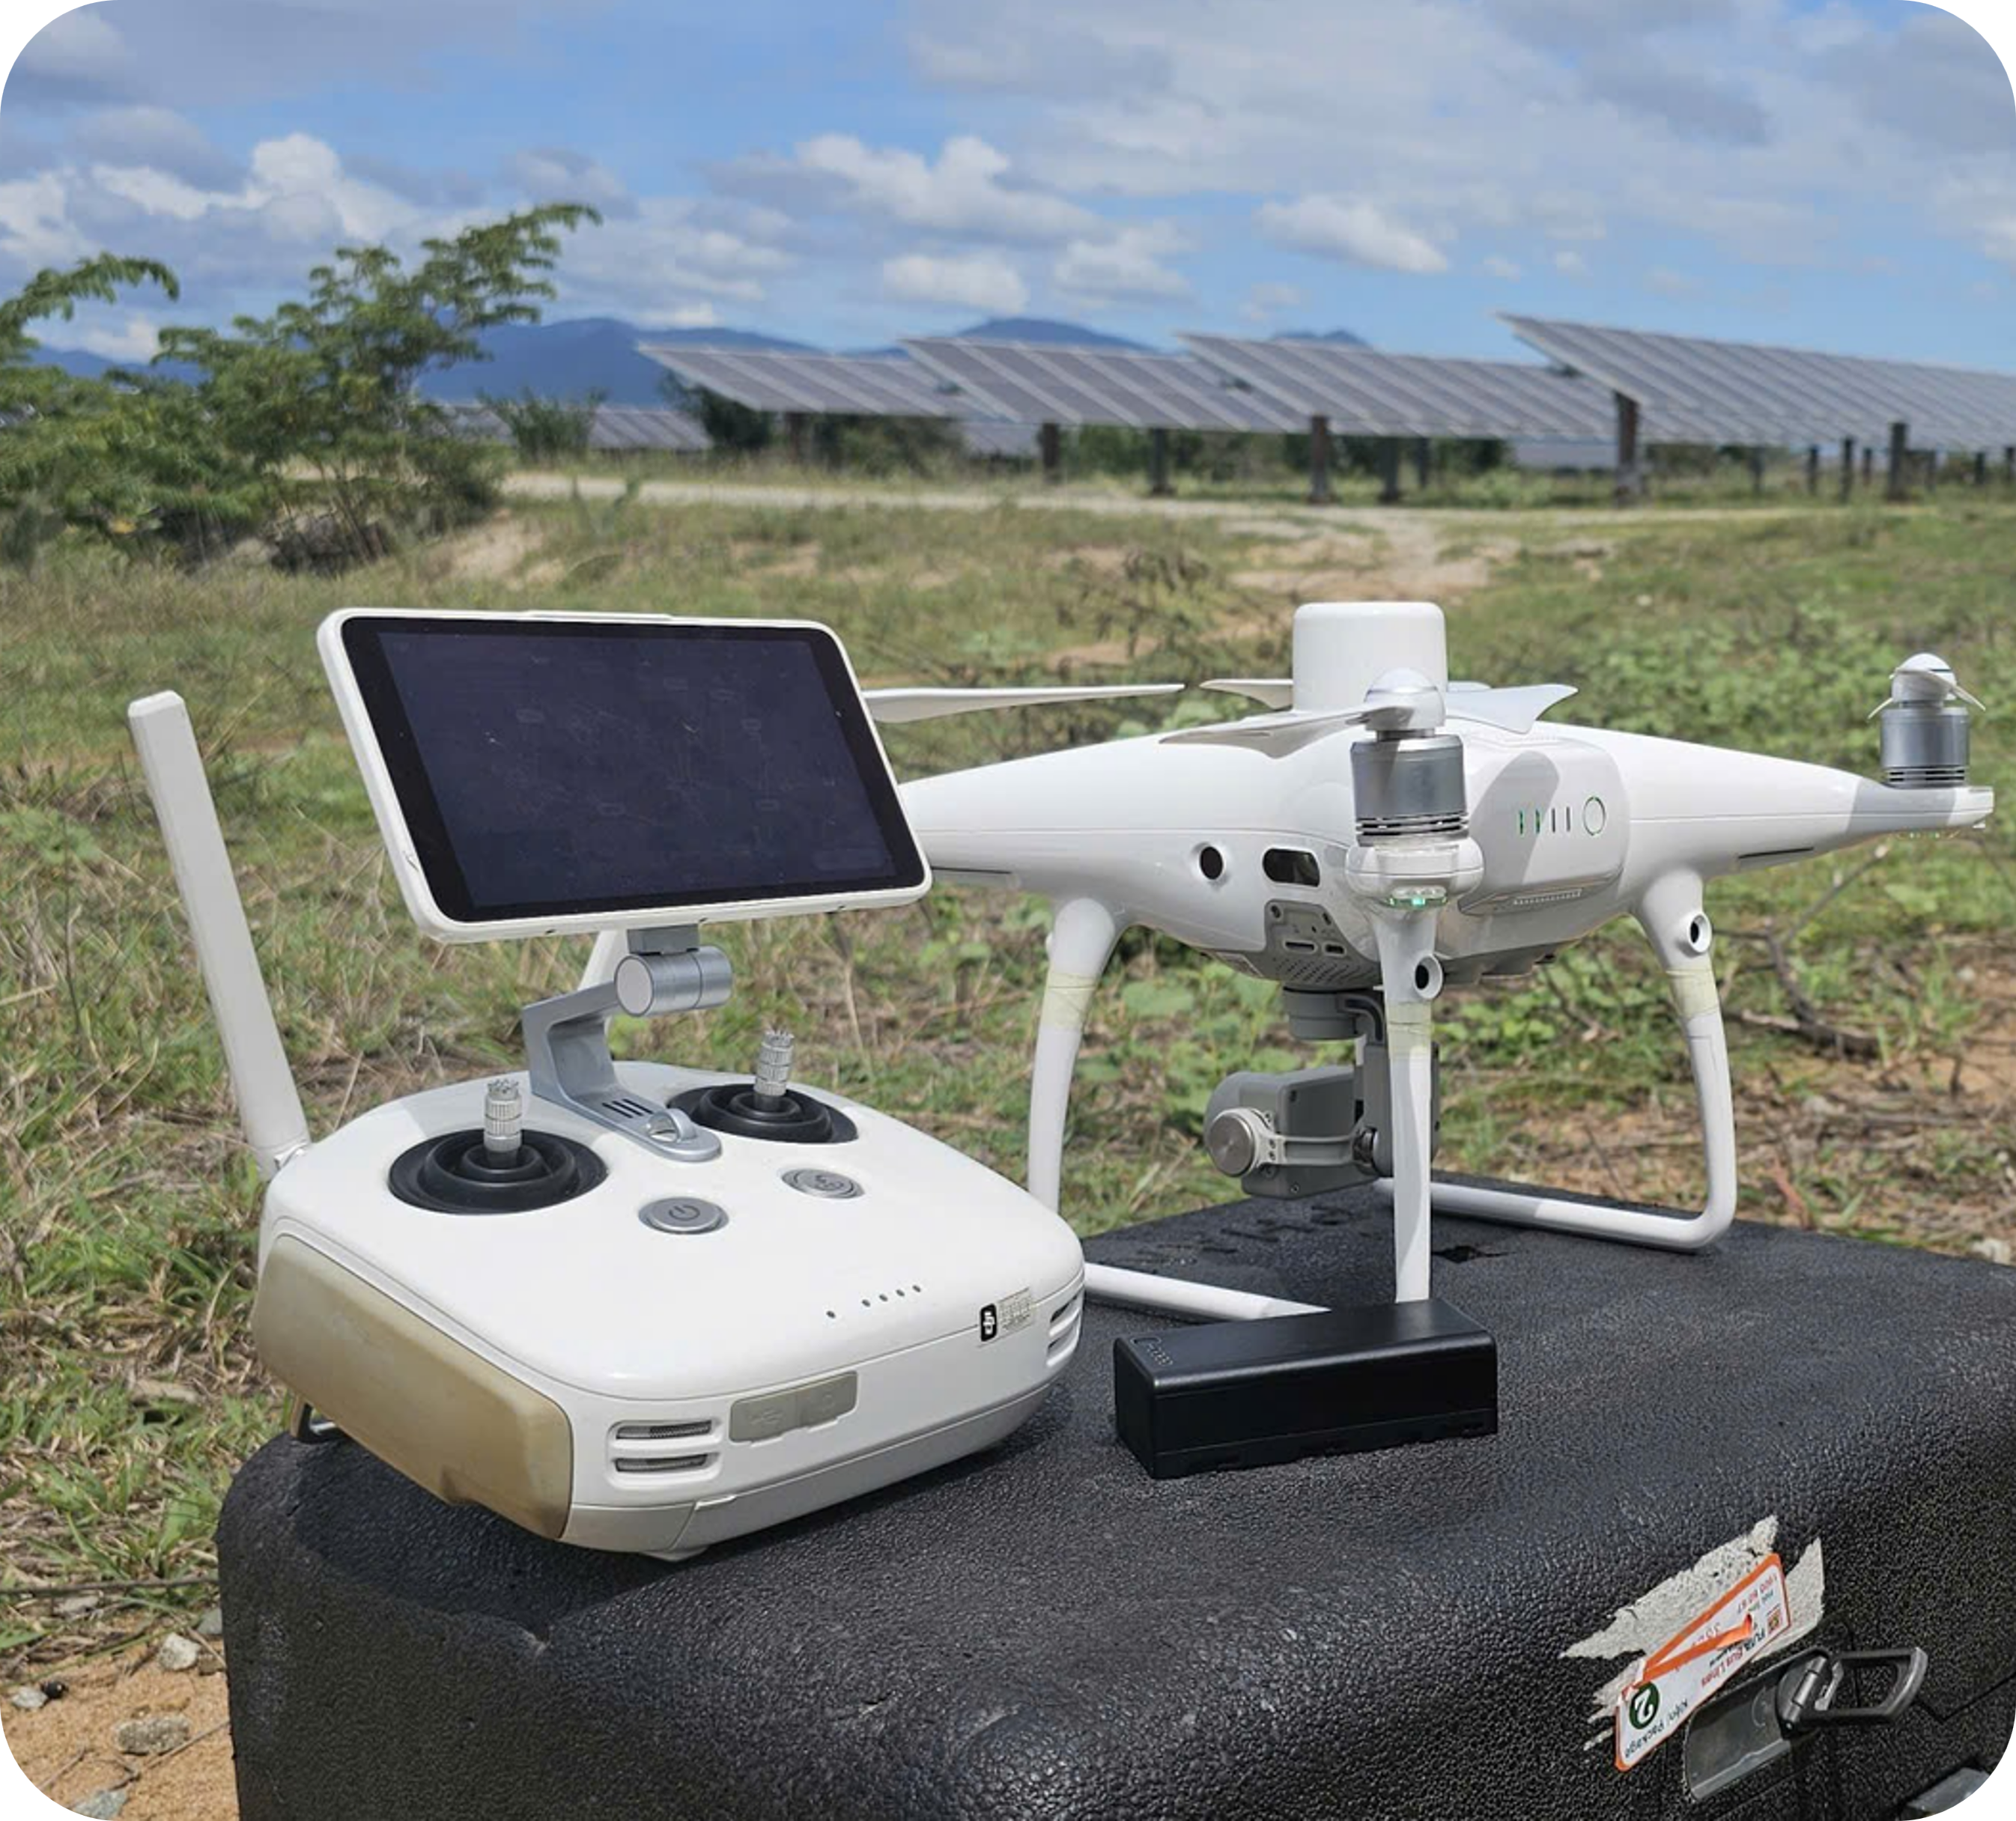
\includegraphics[width=1.7\linewidth]{images/PhuongPhap/uav.png}};
            \end{tikzpicture}
        \end{column}
    \end{columns}
\end{frame}

% Slide hinhminhhoa da duoc gop vao slide tren


\begin{frame}
    \frametitle{ĐỊA ĐIỂM THU THẬP DỮ LIỆU UAV}
    
    \vspace{0.2cm}

    \begin{columns}[c, onlytextwidth]
        % --- CỘT TRÁI: NỘI DUNG ---
        \begin{column}{0.55\textwidth}
            \centering
            % Tên nhà máy - In đậm, màu #151c55, IN HOA
            {\Large \textbf{\textcolor[HTML]{151C55}{NHÀ MÁY ĐIỆN MẶT TRỜI ADANI PHƯỚC MINH}}}
            
            \vspace{0.3cm}
            % Dải phân cách
            {\color{gray!70}\rule{0.3\linewidth}{2pt}}
            \vspace{0.3cm}
            
            % Địa chỉ
            {\large Đ/C: Thôn Quán Thẻ 1, xã Thuận Nam, tỉnh Khánh Hòa.}
        \end{column}

        % --- CỘT PHẢI: HÌNH ẢNH ---
        \begin{column}{0.42\textwidth}
            \centering
            \begin{tikzpicture}
                % Bo góc tròn
                \clip [rounded corners=12pt] (0,0) rectangle (\linewidth, 5.5cm);
                \node[anchor=south west, inner sep=0pt] at (0,0) {
                    \includegraphics[width=\linewidth, height=5.5cm, keepaspectratio=false]{images/PhuongPhap/diadiem.jpg}
                };
                % Thêm viền mỏng cho đẹp nếu cần
                % \draw[rounded corners=12pt, line width=1pt, gray!50] (0,0) rectangle (\linewidth, 5.5cm);
            \end{tikzpicture}
        \end{column}
    \end{columns}
\end{frame}



\begin{frame}
\label{toancanh}
	\frametitle{THÔNG SỐ BAY TỐI ƯU}
	
    \vspace{0.2cm}

    % --- DÒNG 1: THÔNG SỐ (1 HÀNG NGANG) ---
    \begin{center}
        \small
        % Icon được hạ thấp xuống để cân giữa với dòng chữ
        \raisebox{-0.3em}{\includegraphics[height=1.2em]{images/PhuongPhap/icons/docao.png}} \textbf{Độ cao:} 25m
        \hspace{0.25cm} \textcolor{gray}{\rule[-0.3em]{1.5pt}{1.2em}} \hspace{0.25cm} % Đường kẻ đứng đậm hơn chút và cân giữa
        \raisebox{-0.3em}{\includegraphics[height=1.2em]{images/PhuongPhap/icons/gocchup.png}} \textbf{Góc chụp:} Vuông góc ($\approx 90^\circ$)
        \hspace{0.25cm} \textcolor{gray}{\rule[-0.3em]{1.5pt}{1.2em}} \hspace{0.25cm}
        \raisebox{-0.3em}{\includegraphics[height=1.2em]{images/PhuongPhap/icons/thoigian.png}} \textbf{Thời gian:} 9:00 - 11:00
    \end{center}

    \vspace{0.3cm}

    % --- DÒNG 2: 2 ẢNH BẰNG NHAU ---
    \begin{columns}[c, onlytextwidth]
        % Ảnh 1: sodobay2.jpg (Màn hình điều khiển)
        \begin{column}{0.49\textwidth}
            \centering
            \begin{tikzpicture}
                % Khung bo góc tròn, chiều cao 5.0cm (cố định để 2 ảnh bằng nhau)
                \clip [rounded corners=12pt] (0,0) rectangle (\linewidth, 5.0cm);
                % Zoom ảnh để lấp đầy khung
                \node[anchor=center] at (0.5\linewidth, 2.5cm) {
                    \includegraphics[width=\linewidth, height=5.0cm, keepaspectratio=false]{images/PhuongPhap/sodobay2.jpg}
                };
            \end{tikzpicture}
        \end{column}
        
        \hfill

        % Ảnh 2: toancanh.jpg (Toàn cảnh bay)
        \begin{column}{0.49\textwidth}
            \centering
            \begin{tikzpicture}
                \clip [rounded corners=12pt] (0,0) rectangle (\linewidth, 5.0cm);
                \node[anchor=center] at (0.5\linewidth, 2.5cm) {
                    \includegraphics[width=1.6\linewidth]{images/PhuongPhap/toancanh.jpg}
                };
            \end{tikzpicture}
        \end{column}
    \end{columns}
\end{frame}

\begin{frame}
\label{anhthuthapboiuav}
	\frametitle{ẢNH THU THẬP BỞI UAV}
	\begin{center}
		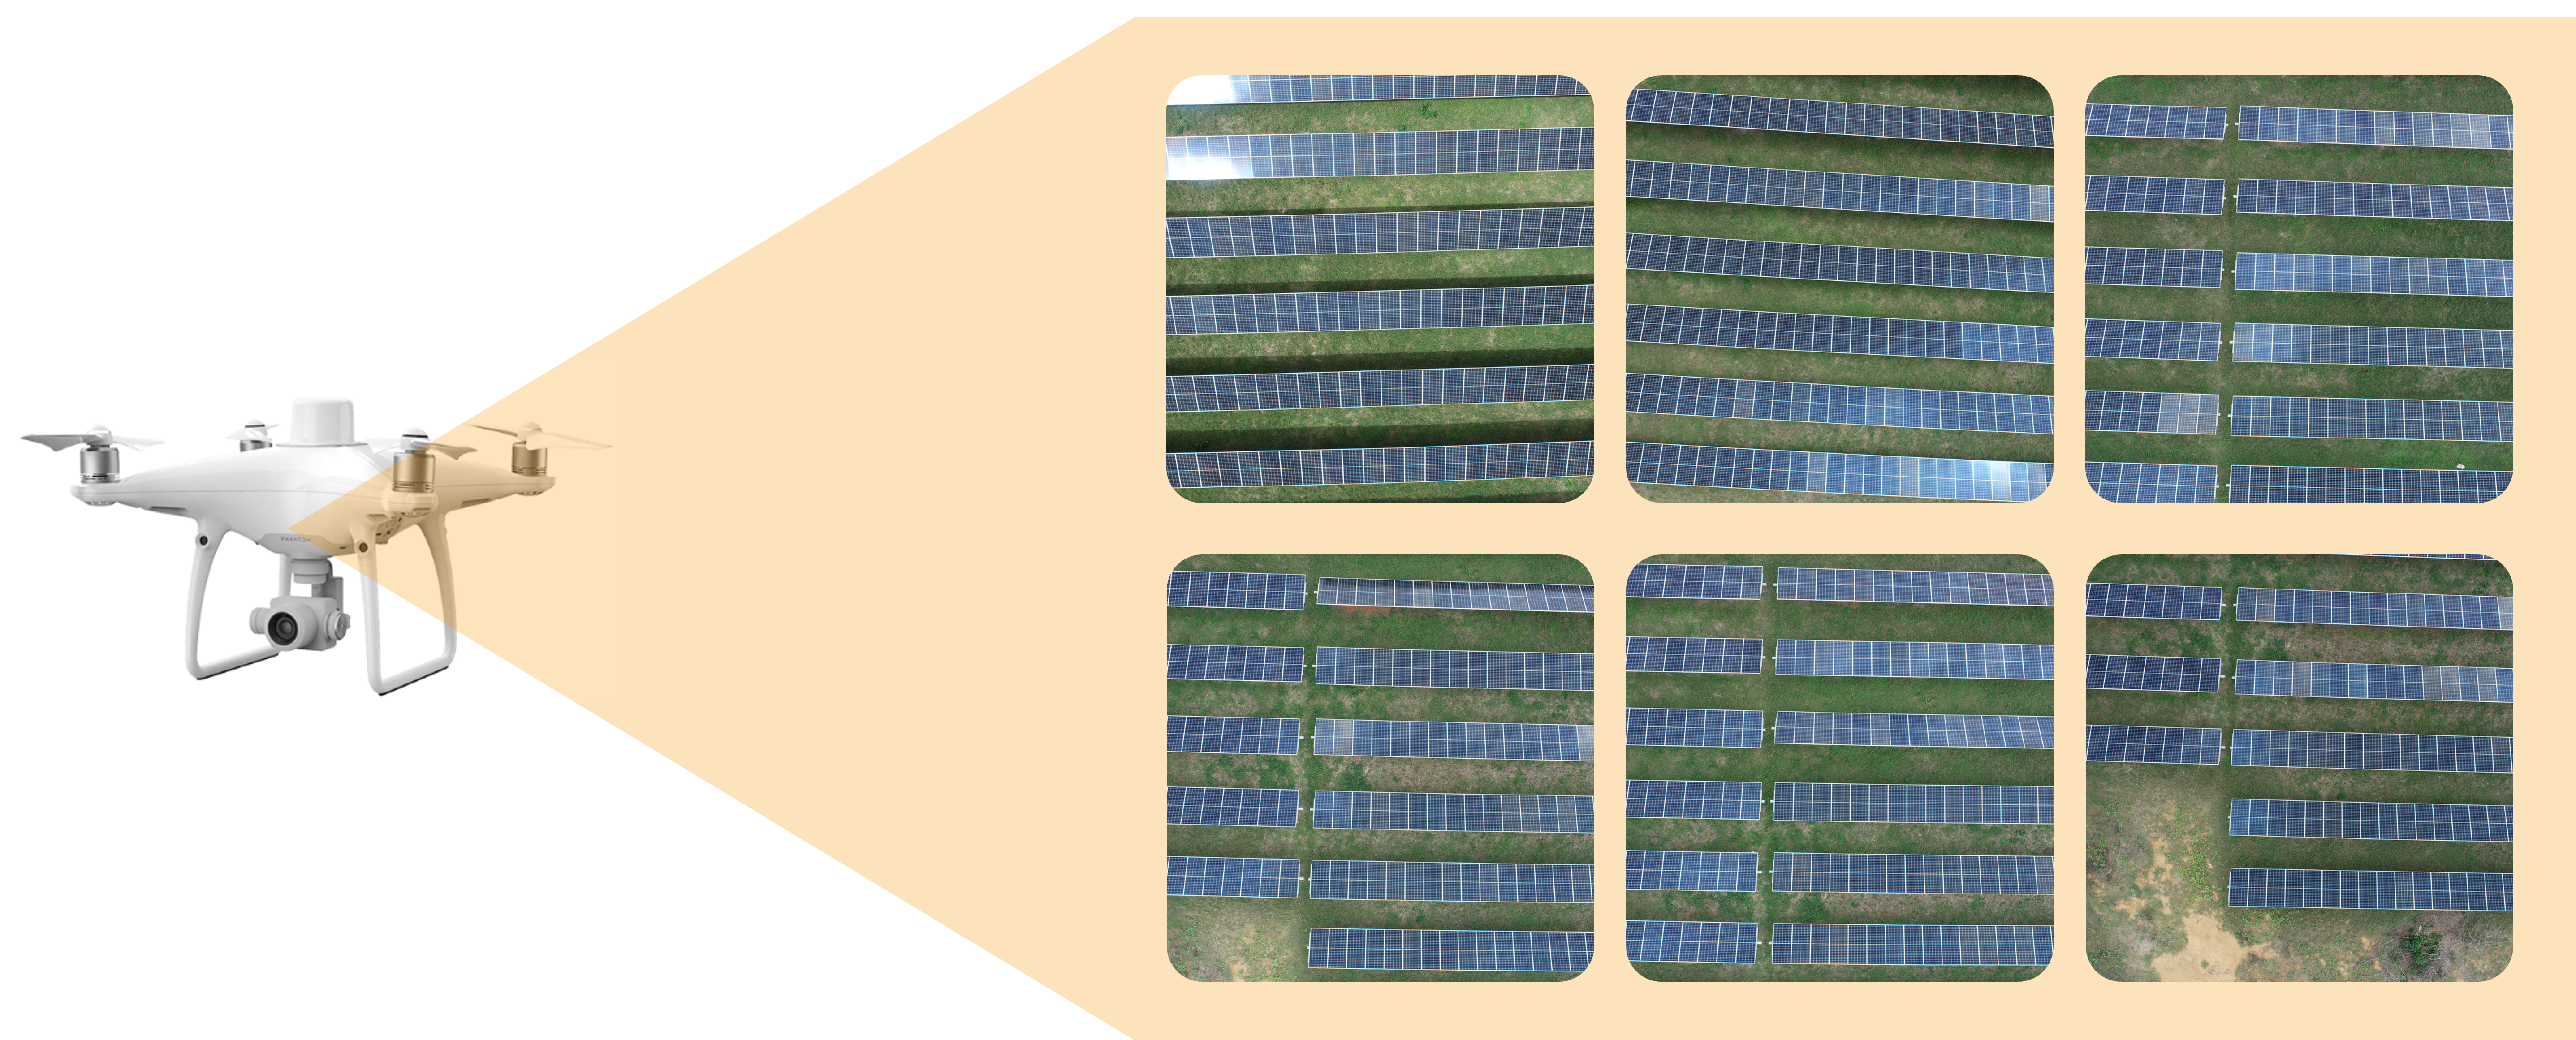
\includegraphics[width=0.7\textwidth]{images/PhuongPhap/thuthap.png}
        
        % Box Kết quả
        \begin{tcolorbox}[
            enhanced,
            title=Kết quả,
            coltitle=white,
            fonttitle=\bfseries\small, 
            colback=bglight,
            colframe=borderblue,
            attach boxed title to top left={xshift=0mm, yshift*=-2mm}, 
            boxed title style={colback=borderblue, sharp corners, rounded corners=southeast, arc=3pt, size=small}, 
            boxrule=0.5pt,
            arc=3pt,
            width=0.9\textwidth,
            left=2mm, right=2mm, top=6pt, bottom=2mm, 
            boxsep=1pt
        ]
            \small 130 ảnh quang học độ phân giải cao, sắc nét, có tọa độ chính xác.
        \end{tcolorbox}
	\end{center}
\end{frame}


\definecolor{myblue}{HTML}{0F52BA} % Màu xanh dương cho số liệu
\definecolor{mypinred}{HTML}{D93025} % Màu đỏ cho cái ghim
\definecolor{mybg}{HTML}{EFF1F3} % Màu xám nhạt nền box

\begin{frame}       
\frametitle{TÁCH CHIẾT TẤM PIN}

\centering

% Phần hình ảnh và nhãn đè lên (Overlay text)
\begin{tikzpicture}
    % Chèn ảnh gốc
    \node[anchor=south west, inner sep=0] (image) at (0,0) {
        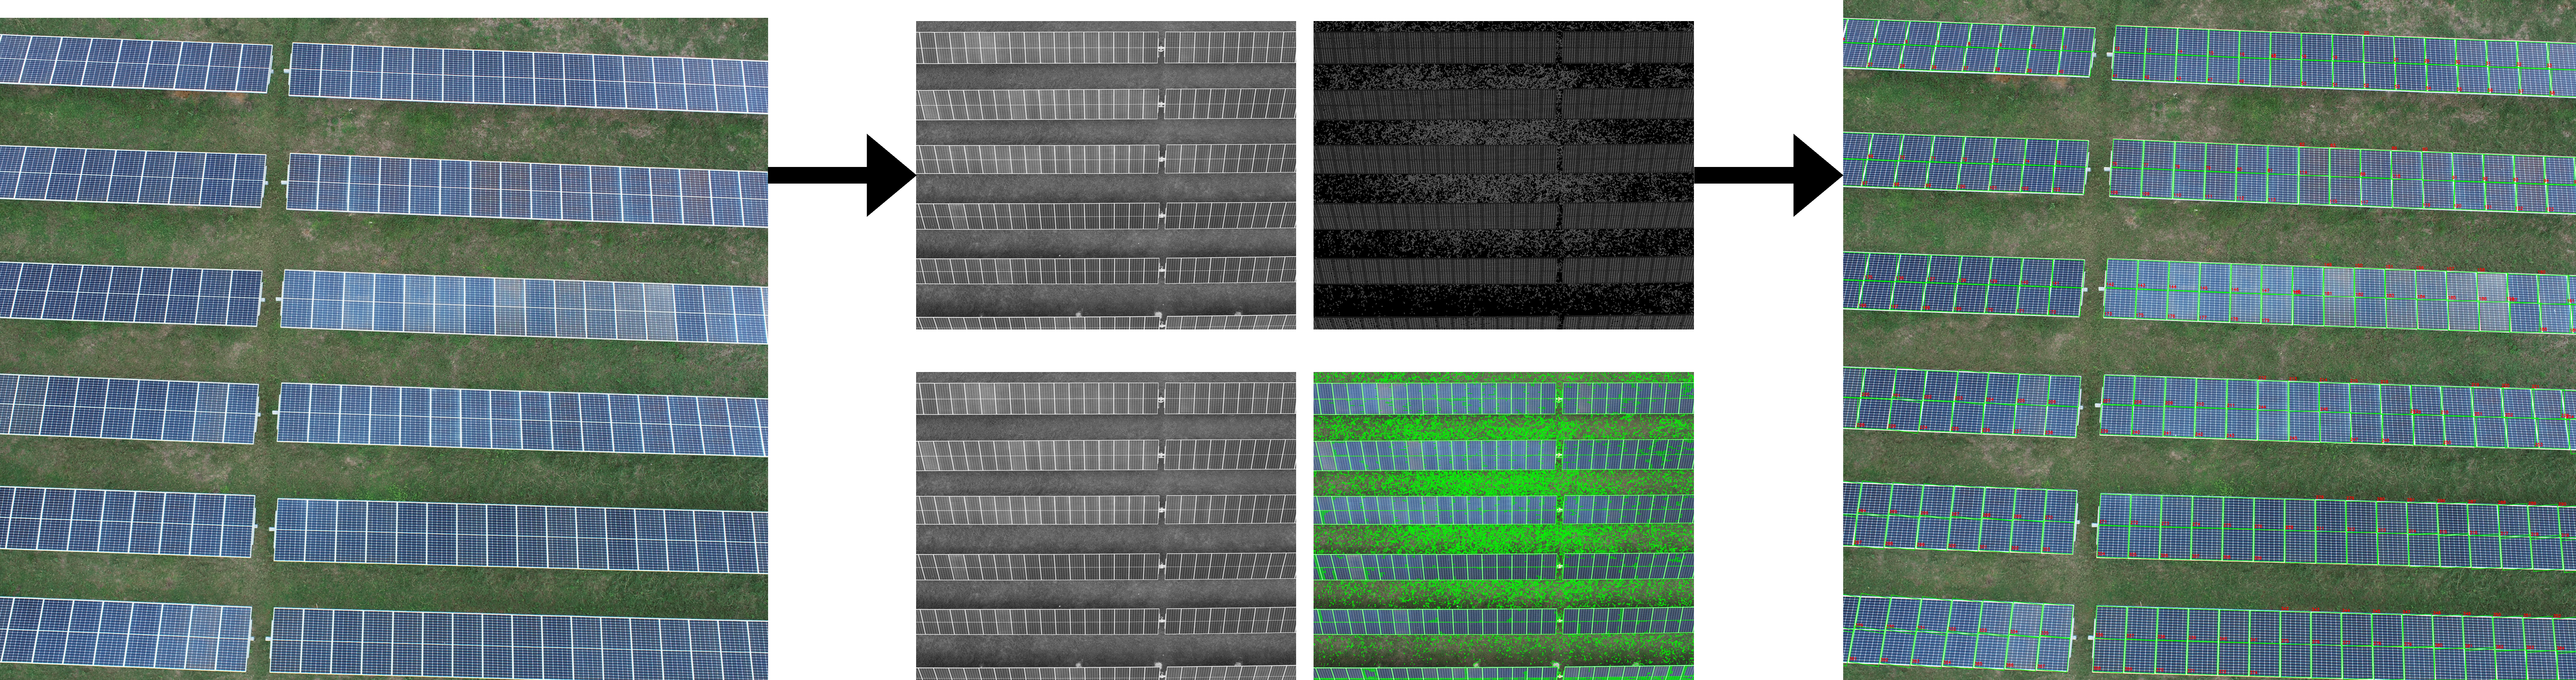
\includegraphics[width=\textwidth]{images/PhuongPhap/tachchiet.png}
    };
    
    % --- PHẦN CHỈNH SỬA VỊ TRÍ NHÃN ---
    % Đã đổi \tiny thành \footnotesize để chữ rõ hơn
\begin{scope}[x={(image.south east)}, y={(image.north west)}, font=\bfseries\fontsize{5pt}{5pt}\selectfont]
    
    % --- HÀNG TRÊN (Điều chỉnh Y xuống khoảng 0.92) ---
    
    % Nhãn: Ảnh GRAY (Góc trên trái - Cột trái)
    \node[anchor=north west, text=white] at (0.265, 1.02) { 
        \textcolor{mypinred}{\faThumbtack}~Ảnh GRAY:
    };
    
    % Nhãn: Ảnh CANNY (Góc trên phải - Cột phải)
    \node[anchor=north west, text=white] at (0.38, 1.02) { 
        \textcolor{mypinred}{\faThumbtack}~Ảnh CANNY:
    };
    
    % --- HÀNG DƯỚI (Điều chỉnh Y xuống khoảng 0.42) ---
    
    % Nhãn: Ảnh BLUR (Góc dưới trái - Cột trái)
    \node[anchor=north west, text=white] at (0.265, 0.51) { 
        \textcolor{mypinred}{\faThumbtack}~Ảnh BLUR:
    };
    
    % Nhãn: Ảnh CONTOUR (Góc dưới phải - Cột phải)
    \node[anchor=north west, text=white] at (0.37, 0.51) { 
        \textcolor{mypinred}{\faThumbtack}~Ảnh CONTOUR:
    };

    % Nhãn: ID trên mũi tên (Giữa ảnh 3 và 4)
    \node[anchor=south] at (0.78, 0.55) { 
        \textbf{\textcolor{red}{\shortstack{ID \\ tương ứng}}}
    };
\end{scope}
\end{tikzpicture}

    \vspace{0.35cm}
    
    % Phần hộp nội dung kết quả (Giữ nguyên)
    \begin{tikzpicture}
        \node[
            fill=mybg, 
            rounded corners=5pt, 
            inner sep=8pt,
            text width=0.94\textwidth,
            anchor=north
        ] {
            \begin{columns}[c]
                \begin{column}{0.3\textwidth}
                    \hspace{0.4cm}\textbf{\textcolor{mypinred}{Kết quả và độ tin cậy}}
                \end{column}
                \begin{column}{0.7\textwidth}
                    \small
                    Quy trình đạt độ chính xác tách chiết \textbf{\textcolor{myblue}{96.9\%}} (Kiểm tra thủ công trên 1.000 mẫu)
                \end{column}
            \end{columns}
        };
    \end{tikzpicture}

\end{frame}

% Định nghĩa màu sắc giống trong ảnh
\definecolor{customRed}{HTML}{FF3333} % Màu đỏ tươi cho số liệu
\definecolor{customGreen}{HTML}{2ECC71} % Màu xanh lá cho dấu check
\definecolor{customGray}{HTML}{CCCCCC} % Màu xám cho đường kẻ dọc

\begin{frame}
    \frametitle{BỘ DỮ LIỆU THỰC NGHIỆM}

    \vspace{0.5cm} % Căn chỉnh khoảng cách từ tiêu đề xuống nội dung

    \begin{columns}[T] % Căn lề trên (Top align) cho các cột
        
        % --- CỘT TRÁI (Số liệu tổng) ---
        \begin{column}{0.35\textwidth}
            \centering
            \vspace{0.5cm} % Đẩy nội dung xuống một chút cho cân giữa
            
            {\Large 130 ảnh UAV} \\[10pt]
            
            % Số to màu đỏ
            {\color{customRed}\textbf{\fontsize{45}{50}\selectfont 5.902}} \\[10pt]
            
            {\large Tổng số ảnh tấm pin}
        \end{column}

        % --- ĐƯỜNG KẺ DỌC ---
        \begin{column}{0.05\textwidth}
            \centering
            % Vẽ đường kẻ dọc màu xám
            {\color{customGray}\vrule width 1.5pt height 4.5cm}
        \end{column}

        % --- CỘT PHẢI (Chi tiết phân bố) ---
        \begin{column}{0.6\textwidth}
            \begin{itemize}
                \setlength\itemsep{1.5em} % Khoảng cách giữa các mục chính
                
                % Mục 1
                \item[\color{customGreen}\Huge\checkmark] 
                    {\large \textbf{Phân bố nhãn:} 3.047 Bình thường / 2.854 Lỗi}
                
                % Mục 2
                \item[\color{customGreen}\Huge\checkmark] 
                    {\large \textbf{Chia tập dữ liệu:}}
                    \vspace{0.3cm}
                    \begin{itemize}
                        \setlength\itemsep{0.5em} % Khoảng cách các mục con
                        \normalsize
                        \item Training: 70\% - 4.131
                        \item Validation: 15\% - 885
                        \item Test: 15\% - 886
                    \end{itemize}
            \end{itemize}
        \end{column}
        
    \end{columns}
\end{frame}


% \begin{frame}
%     \frametitle{TĂNG CƯỜNG DỮ LIỆU}
%     \centering
    
%     % Thiết lập chiều rộng của cột (gần một nửa slide trừ đi khoảng đệm)
%     \newcommand{\colW}{0.46\textwidth}
%     % Thiết lập CHIỀU CAO CỐ ĐỊNH cho mỗi ô (QUAN TRỌNG ĐỂ KHÔNG BỊ DÃN)
%     \newcommand{\rowH}{3.2cm} 
%     % Thiết lập chiều cao ảnh tối đa
%     \newcommand{\imgH}{2.0cm}

%     % Bắt đầu bảng với các đường kẻ | ở giữa
%     \begin{tabular}{c|c}
    
%         % --- GÓC TRÊN TRÁI ---
%         \begin{minipage}[c][\rowH][c]{\colW}
%             \centering
%             \textbf{Xoay (Rotation): +/- 15$^\circ$} \\ 
%             \vspace{2pt} % Khoảng cách rất nhỏ
%             \includegraphics[height=\imgH, keepaspectratio]{images/PhuongPhap/dataaugment/rotation.png}
%         \end{minipage}
%         & 
%         % --- GÓC TRÊN PHẢI ---
%         \begin{minipage}[c][\rowH][c]{\colW}
%             \centering
%             \textbf{Lật (Flip): Ngang/Dọc} \\ 
%             \vspace{2pt}
%             \includegraphics[height=\imgH, keepaspectratio]{images/PhuongPhap/dataaugment/flip.png}
%         \end{minipage}
%         \\ 
%         \hline % ĐƯỜNG KẺ NGANG LIỀN MẠCH
        
%         % --- GÓC DƯỚI TRÁI ---
%         \begin{minipage}[c][\rowH][c]{\colW}
%             \centering
%             \vspace{2pt} % Đẩy nhẹ nội dung xuống khỏi đường kẻ
%             \textbf{Color Jitter: Độ Sáng/Tương Phản} \\ 
%             \vspace{2pt}
%             \includegraphics[height=\imgH, keepaspectratio]{images/PhuongPhap/dataaugment/color.png}
%         \end{minipage}
%         & 
%         % --- GÓC DƯỚI PHẢI ---
%         \begin{minipage}[c][\rowH][c]{\colW}
%             \centering
%             \vspace{2pt}
%             \textbf{Noise Injection: Nhiễu Gaussian} \\ 
%             \vspace{2pt}
%             \includegraphics[height=\imgH, keepaspectratio]{images/PhuongPhap/dataaugment/noise.png}
%         \end{minipage}
        
%     \end{tabular}
% \end{frame}

% --- MÀU SẮC ---
\definecolor{myBlueLine}{HTML}{0072BC}
\definecolor{myBlueBack}{HTML}{F0F6FA}
\definecolor{myOrangeLine}{HTML}{F7941D}
\definecolor{myOrangeBack}{HTML}{FFF9F0}

% --- STYLE KHUNG (Đã thu gọn padding) ---
\tcbset{
    myboxstyle/.style={
        enhanced,
        boxrule=0pt,
        leftrule=0pt,
        arc=3pt,
        auto outer arc,
        % GIẢM PADDING ĐỂ TIẾT KIỆM CHỖ
        left=6pt, right=6pt, top=5pt, bottom=5pt, 
        boxsep=0pt,
    }
}

% % Thêm tùy chọn [shrink] để Beamer tự động co nhỏ nếu vẫn bị tràn
\begin{frame} 
    \frametitle{CHIẾN LƯỢC HUẤN LUYỆN}

    \vspace{-0.2cm} 
    % --- KHỐI KỸ THUẬT (DƯỚI) ---
    \begin{tcolorbox}[
        myboxstyle,
        colback=myOrangeBack,
        colframe=myOrangeLine,
        width=\textwidth
    ]
        \small 
        \begin{center}
            \textbf{Kỹ Thuật}
        \end{center}
        \vspace{-8pt}

        \begin{itemize}
            \setlength\itemsep{2pt} 
            \item \textbf{Augmentation:} Xoay, Lật, Chỉnh màu, Nhiễu Gaussian.
            \item \textbf{Optimizer:} Adam (LR $1e-4$).
            \item \textbf{Early Stopping:} Patience = 5.
            \item \textbf{Loss:} Weighted Cross-Entropy.
        \end{itemize}
    \end{tcolorbox}

\end{frame}
